\clearpage
\section{Separating grid, time and settling effects}\label{sec:accuracy}
All measurements in this section are generated by \code{scripts/run\_accuracy.py}
and retained in \code{data/accuracy.json}. They use the same cavity equations,
wall treatment and interior stencils as the production study.

\subsection{A three-grid estimate independent of the benchmarks}
For $\Rey=400,1000$ use $N=65,129,257$. For $\Rey=3200$ use
$N=129,193,257$, avoiding the very coarse $65^2$ grid in the order estimate.
Each state starts from rest and reaches the same steady threshold. Write
$h_c>h_m>h_f$ for the coarse, medium and fine spacings. For a scalar observable
$q$, assume a leading error model
\begin{equation}
q(h)=q_0+C h^p,\qquad
\frac{q_c-q_m}{q_m-q_f}
=\frac{h_c^p-h_m^p}{h_m^p-h_f^p}.\label{eq:richardson}
\end{equation}
The latter equation is solved for $p$ using the actual spacings; no equal-ratio
formula is imposed on the $\Rey=3200$ sequence. It gives
\begin{equation}
q_0^{\rm est}=q_f+\frac{q_f-q_m}{(h_m/h_f)^p-1},\qquad
U_h=1.25\frac{|q_f-q_m|}{(h_m/h_f)^p-1}.
\end{equation}
The corresponding relative grid-convergence index is $100U_h/|q_f|$,
following the three-grid safety factor of Celik et al.~\cite{celik2008}.
Non-monotone sequences, roundoff-level differences, and sequences with no
positive fitted order in $(0.01,10)$ receive no extrapolation.

\begin{center}\small
\begin{tabular}{@{}rlrrr@{}}\toprule
$\Rey$ & $N$ values & Fitted $p$ & $\psi_{\min,0}^{\rm est}$ & GCI (\%)\\\midrule
\tableinput{grid_rows.tex}
\bottomrule\end{tabular}
\end{center}
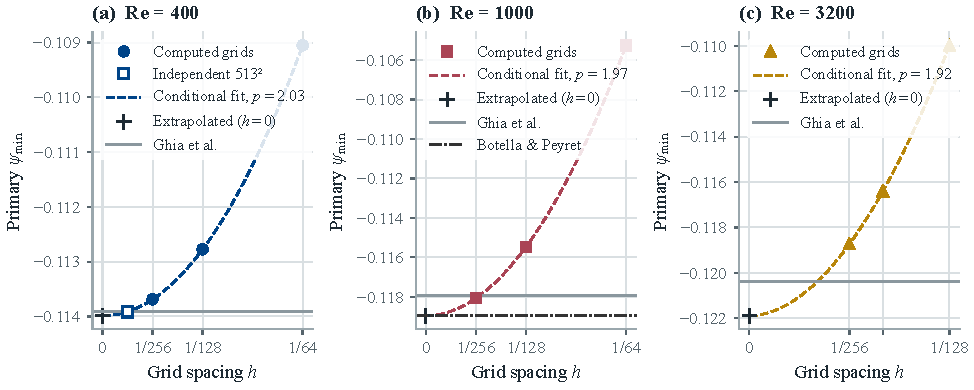
\includegraphics[width=\linewidth]{grid_convergence.pdf}
{\small\color{muted}Computed primary streamfunctions and conditional fits.
The point at $h=0$ is an extrapolation, not an additional simulation.
Reference lines do not enter the fit.}

Three data points determine the three model parameters; a successful fit is
therefore not an independent test of the power-law assumption. These are
engineering uncertainty estimates, not guaranteed bounds or statistical
confidence intervals. The fitted $p$ belongs to this observable and grid range,
not to every quantity produced by the solver.

\clearpage
\subsection{An independent fourth-grid check at Re = 400}
An additional $513^2$ run starts from rest and meets the same stopping
criterion. Comparing overlapping triples tests the original extrapolation:
\begin{center}\small
\begin{tabular}{@{}lrrr@{}}\toprule
$N$ values & Fitted $p$ & Extrapolated $\psi_{\min}$ & Fine-grid GCI (\%)\\\midrule
\tableinput{fourth_grid_rows.tex}
\bottomrule\end{tabular}
\end{center}
The original three-grid model predicts $\psi_{\min}=-0.1139135$ on $513^2$; the independent integration gives $-0.1139144$, a difference of $9.51\times10^{-7}$. The two extrapolated limits differ by $1.67\times10^{-6}$. This is an independent check of the primary-streamfunction model at $\Rey=400$ only. It does not establish the same reliability for other Reynolds numbers or observables.


\subsection{Other observables and complete centerline differences}
The same procedure is applied to the vortex coordinates, kinetic energy,
center vorticity, and bottom-right secondary-vortex strength.

\begin{center}\footnotesize
\begin{tabular}{@{}rlrrl@{}}\toprule
$\Rey$ & Observable & Fitted $p$ & GCI (\%) & Interpretation\\\midrule
\tableinput{observable_rows.tex}
\bottomrule\end{tabular}
\end{center}

Profile differences use 65 common, uniformly spaced grid nodes, including
the endpoints; no interpolation is needed. Their $L^2$ norm uses composite
trapezoidal integration on $[0,1]$, distinct from the RMS over Ghia's
17 irregularly spaced stations.

\begin{center}\small
\begin{tabular}{@{}rlrr@{}}\toprule
$\Rey$ & Grid pair & $\|\delta u\|_{2}$ & $\|\delta v\|_{2}$\\\midrule
\tableinput{grid_profile_rows.tex}
\bottomrule\end{tabular}
\end{center}

At $\Rey=400$, the bottom-right eddy strength is non-monotone across the
three grids, so no GCI is assigned. At $\Rey=3200$, the kinetic-energy GCI
is $6.695\%$, versus $3.321\%$ for the primary streamfunction. Position
estimates also depend on the local quadratic fit used to locate the extremum.

\takeaway{The main vortex's uncertainty estimate cannot be transferred to
secondary eddies or to the whole velocity field.}

\clearpage
\subsection{Time refinement at a common transient time}
For each Reynolds number, integrate afresh from rest on the same $129^2$ grid
to $T=5$ with $\dt$, $\dt/2$, and $\dt/4$. The target is an integer multiple
of every step. Define
\begin{equation}
D_u(\dt)=\|u_{\dt}(1/2,\cdot,T)-u_{\dt/2}(1/2,\cdot,T)\|_2,
\quad p_{t,u}=\log_2\frac{D_u(\dt)}{D_u(\dt/2)},
\end{equation}
and similarly for $v$. Using a common grid isolates temporal self-convergence
from spatial refinement. It does not measure the continuum error at that grid.

\begin{center}\small
\begin{tabular}{@{}rrrrrr@{}}\toprule
$\Rey$ & Base $\dt$ & $D_u(\dt)$ & $D_u(\dt/2)$ & $p_{t,u}$ & $p_{t,v}$\\\midrule
\tableinput{time_rows.tex}
\bottomrule\end{tabular}
\end{center}
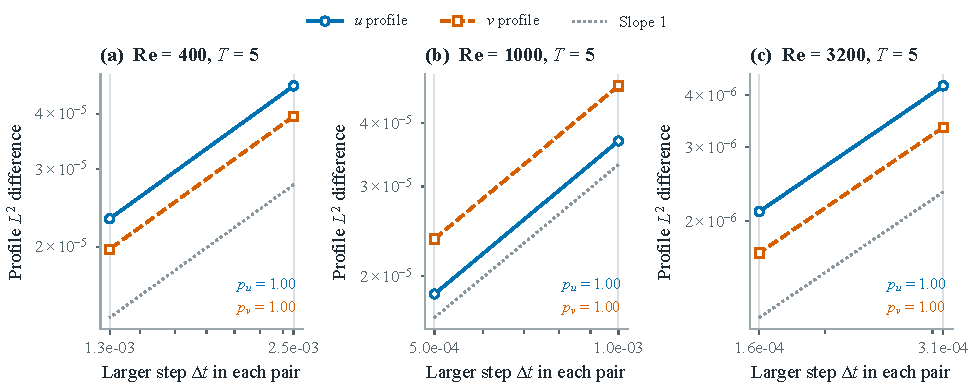
\includegraphics[width=\linewidth]{cavity_time_convergence.pdf}
{\small\color{muted}Successive profile differences from actual cavity
transients. All runs use the impulsively started, discontinuous unit lid.}

\subsection{Why a steady solution has a different time-step question}
At an exactly stationary discrete state, $\omega^{n+1}=\omega^n=\omega$
and the lagged boundary is also stationary. Subtracting $\omega$ from
\eqref{eq:step} and dividing by $\dt$ gives
\begin{equation}
C_h(\psi,\omega)-\Rey^{-1}\Delta_h\omega=0.
\end{equation}
Thus the time step cancels out of the fixed-point equations. There is no
separate backward-Euler truncation bias in their exactly converged solution.
The step still affects transient accuracy, stability, and how closely the
iteration approaches that fixed point. Different stable steps can also have
different attraction behavior if multiple discrete solutions exist.

This is why the time-order experiment is performed during the transient.
For the final states, halving the step is instead used as a continuation
sensitivity check, together with an unfiltered steady-equation residual.

\clearpage
\subsection{Measure settling instead of relying only on a threshold}
Refresh the wall vorticity from the current $\psi$ and evaluate
\begin{equation}
F_h=C_h(\psi,\omega)-\Rey^{-1}\Delta_h\omega,\qquad
R_{\rm PDE}=\|F_h\|_\infty.
\end{equation}
The monitored update rate is related to the old-state defect by
$(I+\dt\Rey^{-1}L)(\omega^{n+1}-\omega^n)/\dt=-F_h$.
It is therefore a filtered residual, not numerically identical to $R_{\rm PDE}$.

Starting independently from each saved final state, integrate ten further
time units with the original step and with half that step. The following
table reports the initial steady defect, the largest monitored update rate
across both continuations, and the larger observable drift of the two trials.
Halving the step reduces the implicit filtering, so its initial update rate
can marginally exceed the original stopping threshold even though the initial
fields are identical. These small excursions are retained; the original-step
stopping criterion is not retroactively changed.

\begin{center}\small
\begin{tabular}{@{}rrrrrrr@{}}\toprule
$\Rey$ & Grid & $R_{\rm PDE}$ & $R_{\max}$ & $|\delta\psi_{\min}|$ & $\|\delta u\|_2$ & $\|\delta v\|_2$\\\midrule
\tableinput{settling_rows.tex}
\bottomrule\end{tabular}
\end{center}

This measures sensitivity over a specified interval. It is not a proof that
all later changes are smaller, and the residual is not divided by an
unjustified decay constant to manufacture an error bound.

The fresh fine-grid integrations also save intermediate states. Comparing
the former observation times to the converged states quantifies the effect
that was previously left unresolved:
\begin{center}\small
\begin{tabular}{@{}rrrrr@{}}\toprule
$\Rey$ & Earlier $t$ & $\psi_{\min}$ change (\%) & $\|\delta u\|_2$ & $\|\delta v\|_2$\\\midrule
\tableinput{transient_rows.tex}
\bottomrule\end{tabular}
\end{center}

\begin{center}\small
\begin{tabular}{@{}rrrr@{}}\toprule
$\Rey$ & Grid GCI (\%) & Settling drift (\%) & Step-halving $|\delta\psi_{\min}|$\\\midrule
400 & 0.327 & 1.830e-05 & 5.49e-13\\
1000 & 0.941 & 7.603e-05 & 5.48e-13\\
3200 & 3.321 & 7.843e-05 & 5.01e-13\\
\bottomrule\end{tabular}\end{center}
The three columns are distinct sensitivity measures on the $257^2$ grids, not independent random errors to combine in quadrature. The first assumes a power-law spatial error; the second measures ten-time-unit drift; the last compares the endpoints of the two continuations. The measured settling effects can thus be assessed against spatial sensitivity without treating the residual threshold as an uncertainty estimate.
Across these three fine-grid cases, the conditional grid estimate is at least $1.24\times10^{4}$ times the measured primary-vortex settling drift. Within these experiments, spatial resolution is the dominant measured limitation for primary-vortex strength. This conclusion does not transfer automatically to every flow quantity.


\takeaway{The completed experiments distinguish measured settling, transient
time accuracy, conditional grid uncertainty, and disagreement with a numerical
reference. Each answers a different question about the computed flow.}
